\documentclass{article}

% if you need to pass options to natbib, use, e.g.:
%     \PassOptionsToPackage{numbers, compress}{natbib}
% before loading neurips_2020
\usepackage[english]{babel}
\usepackage[square,numbers]{natbib}
\bibliographystyle{abbrvnat}

% ready for submission
% \usepackage{neurips_2020}

% to compile a preprint version, e.g., for submission to arXiv, add add the
% [preprint] option:
\usepackage[preprint]{neurips_2020}

% to compile a camera-ready version, add the [final] option, e.g.:
%     \usepackage[final]{neurips_2020}

% to avoid loading the natbib package, add option nonatbib:
%     \usepackage[nonatbib]{neurips_2020}

\usepackage[utf8]{inputenc} % allow utf-8 input
\usepackage[T1]{fontenc}    % use 8-bit T1 fonts
\usepackage{hyperref}       % hyperlinks
\usepackage{url}            % simple URL typesetting
\usepackage{booktabs}       % professional-quality tables
\usepackage{amsfonts}       % blackboard math symbols
\usepackage{nicefrac}       % compact symbols for 1/2, etc.
\usepackage{microtype}      % microtypography
\usepackage{graphicx}
\usepackage{mathtools}
\usepackage{caption}
\usepackage{subcaption}
\DeclarePairedDelimiter\ceil{\lceil}{\rceil}
\DeclarePairedDelimiter\floor{\lfloor}{\rfloor}

\title{Transfer Learning on Dog Breed Classification}

% The \author macro works with any number of authors. There are two commands
% used to separate the names and addresses of multiple authors: \And and \AND.
%
% Using \And between authors leaves it to LaTeX to determine where to break the
% lines. Using \AND forces a line break at that point. So, if LaTeX puts 3 of 4
% authors names on the first line, and the last on the second line, try using
% \AND instead of \And before the third author name.

\author{
Zhaokai Xu, Dian Yu \\
Department of Computer Science and Engineering \\
University of California, San Diego \\
La Jolla, CA 92093 \\
\texttt{\{d9yu,xuzhx121\}@eng.ucsd.edu} \\
}

\begin{document}

\maketitle

\begin{abstract}
 Image classification is becoming increasingly important in the digital world and has applications that go far beyond just facial recognition for humans. Image Classification, especially fine-grained image recognition, has important applications in industries ranging from social media to marketing to national security. We want to build a dog breed classifier because dog is one of the most popular animals in American families. Dog breed identification models can be used not only to satisfy our own curiosity, but also help match dogs to owners, return lost dogs to their homes. In order to accomplish our goal of building a dog breed classification model, we use the Stanford Dog Dataset and a variety of transfer learning methods including ResNet34, VGG19, and Inception V3, as well as an baseline CNN model built from scratch.
\end{abstract}

\section{Introduction}
In recent years, deep learning has become increasingly popular in the field of artificial intelligence. Among the considerably rapid improvement of deep learning technology, fine-grained classification such as animal breed classification and facial recognition is highly researched. 

The goal of our project is to build a fine-grained image classification model that classifies dog breeds. Some of the previous work include \cite{dog_breed_classification}. However, achieving a high level of accuracy is a significant challenge due to the large variance in the same subcategory (breed) while also having a small variance between different subcategories. For example, dogs of different breeds could share some similar visible features such as color and hair, while the dogs of the same breed could differ significantly depending on the age, size and color. Therefore, traditional machine learning methods such as K-Nearest Neighbor and Decision Trees might be almost impossible to tackle this type of problem. Instead, we need more powerful models such as neural networks to extract the detailed features and distinguish different dog breeds. 

On the application side, dog classification can help both owners and buyers of dogs. Knowing the breed, or a possible mix of breeds can help to match dogs to families by identifying breeds with certain personality characteristics or physical requirements. Additionally, as the field continues to advance, dog classification models could help identify and automate the process of returning lost dogs to their owners through facial recognition. On the research side, the solution of the problem will also be applicable to other fine-grained classification tasks, such as recognizing bird species and marine animals. In addition, this project tackles on training a deep learning model with relatively limited data, which could help the researches on how to solve a deep learning problem when data is somehow restricted and noisy.

\section{Dataset and Preprocessing}
The dataset we chose is Stanford Dogs Dataset\footnote{http://vision.stanford.edu/aditya86/ImageNetDogs/}, which is introduced by Khosla in 2011\cite{novel_dataset}. It contains 20580 images of dogs belonging to 120 species, divided into 120 folders. The dataset contains both basic picture of dogs as well as some variations of them. For example, there are dogs with clothes on, dogs with human standing aside, or side view of the dog’s face. This high inter-class variance and low intra-class variance among images makes the classification even harder.  

We did a little bit of Exploratory Data Analysis (EDA) in order to get a bird view of the breeds and the images we were going to be working with. Figure \ref{fig:eda} shows the distribution of the dog breeds in this dataset. As we can see, nearly most of the dog breeds have less than 120 (or the number of classes) images, despite the noise those images could have. The limited number of data makes the classification task challenging.
\begin{figure}[h!]
    \centering
    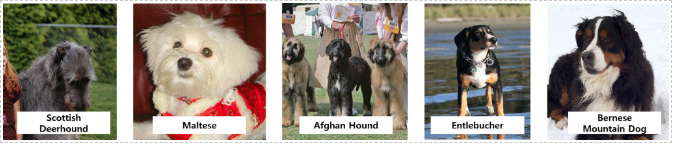
\includegraphics[width=12cm]{dogs.PNG}
    \caption{Some Dogs and Their Breeds}
    \label{fig:dogs}
\end{figure}
\begin{figure}[h!]
    \centering
    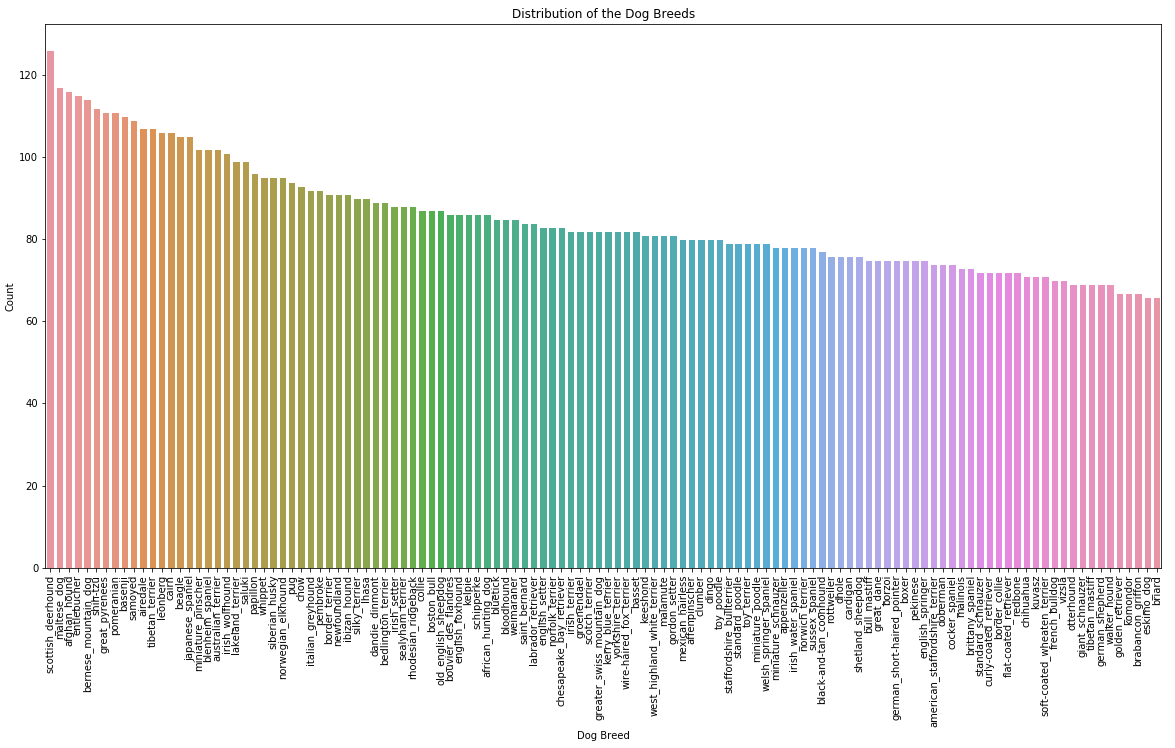
\includegraphics[width=12cm]{eda.PNG}
    \caption{Dog Breeds Count}
    \label{fig:eda}
\end{figure}

To make the task even harder, we partition the dataset into three smaller ones, of each breed with 60, 40, and 20 images, chosen randomly from the original dataset. To train these models, we split the training, validation, and testing sets with a ratio of 4:1:1. In this way, we can test the robustness of our models under the circumstance that there are extremely limited data.

To help build powerful image classifier with very little data, we use data augmentation to perform random cropping, rotation, and flipping on the images. Beside, we normalize the RGB values of each pixel with the means of $0.485, 0.456, 0.406$ and the standard deviations of $0.229, 0.224, 0.225$. In addition, we standardize the sizes of all images to align with the input size of each model we are trying to test (224 by 224 for ResNet and VGG and 299 by 299 for Inception).
\begin{figure}[h!]
    \centering
    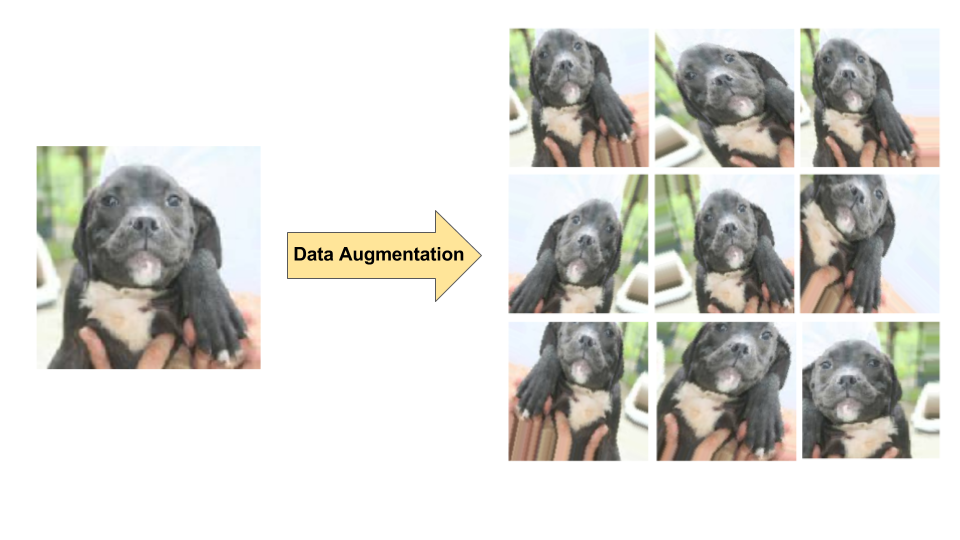
\includegraphics[width=10cm]{data_augmentation.png}
    \caption{Data Augmentation}
    \label{fig:aug}
\end{figure}

\section{Method}
We build a simple Convolutional Neural Network (CNN) as the baseline and use transfer learning on the pre-trained models of ResNet34, VGG19, and Inception V3, all from \textit{Pytorch}
library\footnote{https://pytorch.org/docs/stable/torchvision/models.html}. The details of each model will be described below. 

\subsection{Transfer learning}
Transfer learning is a research problem in machine learning that focuses on storing knowledge gained while solving one problem and applying it to a different but related problem. The main advantage of it is it can save time and computing resources significantly. The idea is initially brought from \cite{transfer_learning}.

If we have significantly more data for task T1, we may utilize its learning, and generalize this knowledge (features, weights) for task T2 (which has significantly less data). In the case of problems in the computer vision domain, certain low-level features, such as edges, shapes, corners and intensity, can be shared across tasks, and thus enable knowledge transfer among tasks. Therefore, We can reuse the weights and biases from previously trained model on a new dataset. In addition, it dramatically shorten the training time since we don’t have to find the features from the scratch.

 \begin{figure}[h!]
    \centering
    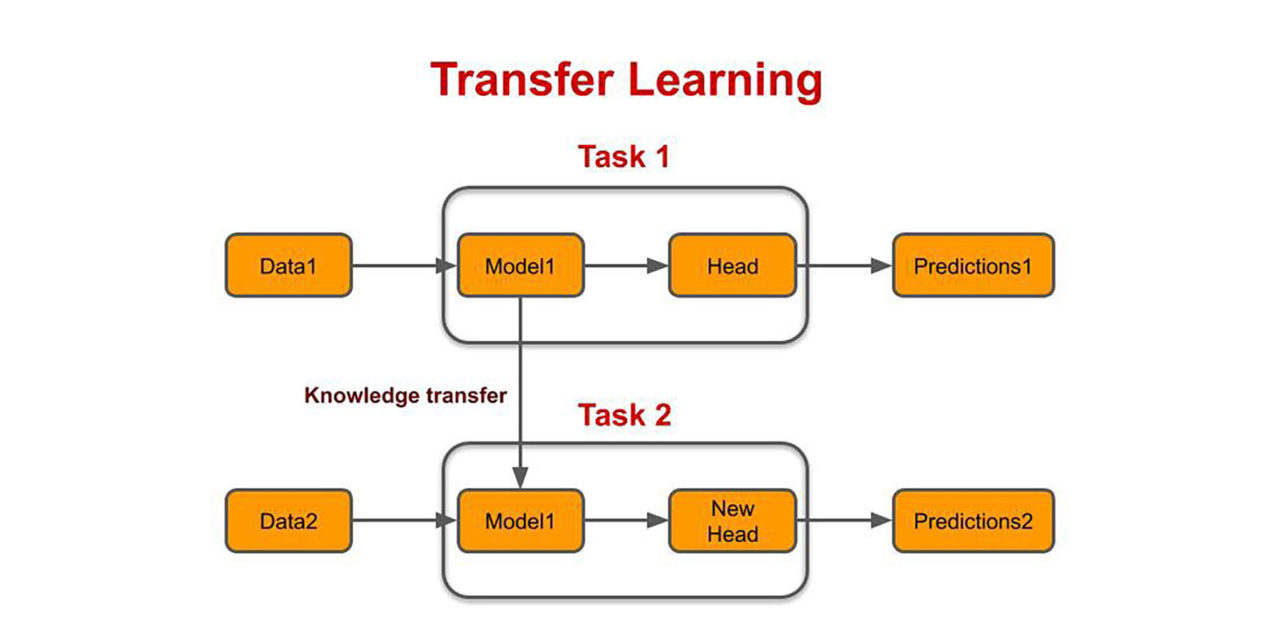
\includegraphics[width=10cm]{transferLearning.jpg}
    \caption{Transfer Learning}
    \label{fig:aug}
\end{figure}


\subsection{Baseline CNN}
As shown at Table \ref{tab:baseline_cnn}, Baseline CNN is constructed with five convolution layers with Batch Normalization, followed by max pooling. The kernel size for each convolution layer is 3x3 with padding of one. In the end, it has two fully connected layers, each with input and output size of 12544 by 512 and 512 by 120. Each fully connected layer is followed by a dropout layer to prevent overfitting. For prediction, We applied a softmax layer to classify the dog breed on its label. For training, we use Cross Entropy Loss as the loss function, as well as Statistical Gradient Descent as the Optimizer. We want the five convolution layers to capture the detailed features of various dogs and make the correct prediction.

\begin{table}[h!]
\centering
\begin{tabular}{ |c||c|c|c|c|c|c| } 
 \hline
 Layer & In-channels & Out-channels & Kernel Size & Padding & Stride & Activation \\ 
 \hline\hline
 Conv2d & 3 & 16 & 3 & 1 & 1 & ReLU\\ 
 \hline
 MaxPool2d & - & - & 2 & 0 & 2  & -\\
 \hline 
 Conv2d & 16 & 32 & 3 & 1 & 1 & ReLU\\ 
  \hline
 MaxPool2d & - & - & 2 & 0 & 2  & -\\
 \hline
  Conv2d & 32 & 64 & 3 & 1 & 1  & ReLU\\ 
   \hline
 MaxPool2d & - & - & 2 & 0 & 2  & -\\
 \hline
 Conv2d & 64 & 128 & 3 & 1 & 1  & ReLU\\ 
  \hline
 MaxPool2d & - & - & 2 & 0 & 2  & -\\
 \hline
  Conv2d & 128 & 256 & 3 & 1 & 1  & ReLU\\ 
 \hline
\end{tabular}
\caption{Baseline CNN Architecture}
\label{tab:baseline_cnn}
\end{table}

\subsection{ResNet34}

Even though InceptionV3 is already good enough for dog classification, we added another model called RestNet34 to this experiment to see the performance of a fast trained deep neural network.

ResNet was the winner of ImageNet challenge in 2015. The fundamental breakthrough with ResNet was it allowed us to train extremely deep neural networks with 150+layers successfully. One of the problems ResNets solve is the famous known vanishing gradient. This is because when the network is too deep, the gradients from where the loss function is calculated easily shrink to zero after several applications of the chain rule. This result on the weights never updating its values and therefore, no learning is being performed. With ResNets, the gradients can flow directly through the skip connections backwards from later layers to initial filters.

 Shown in Figure \ref{fig:resnet}, ResNet34\cite{resnet} contains layers follow the same pattern. They perform 3x3 convolution with a fixed feature map dimension [64, 128, 256, 512] respectively, bypassing the input every 2 convolutions. Furthermore, the width (W) and height (H) dimensions remain constant during the entire layer. Besides, every layer of a ResNet is composed of several blocks. This is because when ResNets go deeper, they normally do it by increasing the number of operations within a block, but the number of total layers remains the same.

%  \begin{figure}[h!]
%     \centering
%     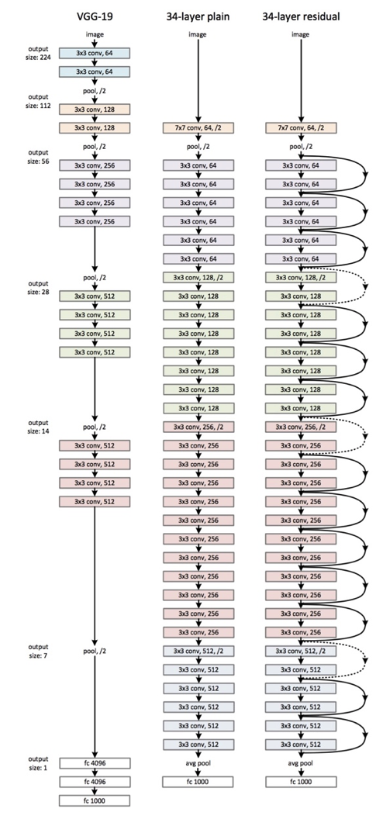
\includegraphics[height=10cm,width=5cm]{vgg19vsResnet34.jpg}
%     \caption{VGG19 vs. ResNet34}
%     \label{fig:vggvsresnet}
% \end{figure}

 \begin{figure}[h!]
    \centering
    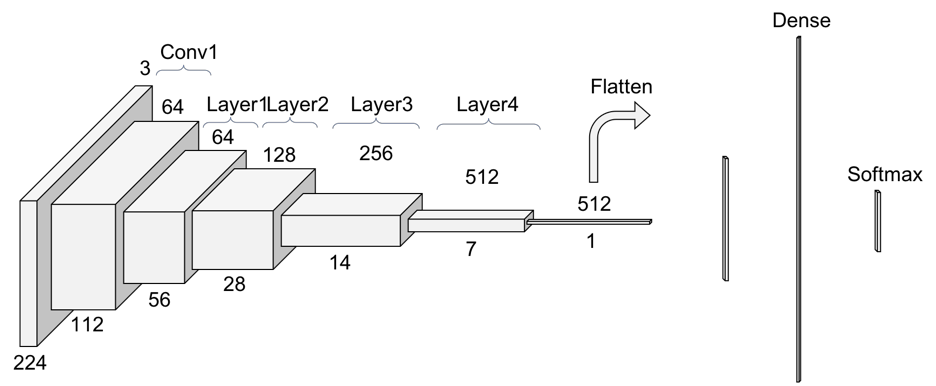
\includegraphics[width=10cm]{restnet34.png}
    \caption{ResNet34}
    \label{fig:resnet}
\end{figure}
    
\subsection{VGG19}
VGG19 is from VGG group, Oxford. It makes the improvement over AlexNet by replacing large kernel-sized filters(11 and 5 in the first and second conv layer) with multiple 3X3 kernel-sized filters one after another. With a given receptive field, multiple stacked smaller size kernel is better than the one with a larger size kernel because multiple non-linear layers increases the depth of the network which enables it to learn more complex features, and that too at a lower cost. 

Shown in Figure \ref{fig:vgg}, the structure of VGG19\cite{vgg} contains 19 convolution layers, 5 max pooling layers and 3 fully connected layers. ReLu function is act as activation function for each convolution layer and fully connected layer, except the last layer. The last layer in the model is a fully connected layer with softmax function. The detail explanation of ReLu function, softmax function can be found in Alexnet model mentioned above. It replace large kernel size with multiple small 3*3 kernel. The benefit of this model is that it can achieve better accuracy than CNN but takes longer time.

 \begin{figure}[h!]
    \centering
    \includegraphics[width=10cm]{VGG.png}
    \caption{VGG19}
    \label{fig:vgg}
\end{figure}

\subsection{Inception V3}
Compared with VGG, even though VGG achieves a phenomenal accuracy on ImageNet dataset, its deployment is problematic because of huge computational requirements, both in terms of memory and time. It becomes inefficient due to large width of convolutional layers. Therefore, we tried the InceptionV3 to improve the training efficiency.

Shown in Figure \ref{fig:inception}, Inception V3\cite{inception}\cite{inception2} is a convolutional neural network for assisting in image analysis and object detection, and originates from Googlenet, but the computation cost is only about 2.5 higher than that of GoogLeNet, and much more efficient than that of VGGNet.

This image recognition model contains 42 layers, and it is mainly divided into two parts, feature extraction with a CNN and a classification aspect with both fully connected and softmax layers. Some major techniques used in Inception V3 are factorizing convolutions, which aims at  reducing the number of connections/parameters without decreasing the network efficiency, and
auxiliary classifiers previously suggested in GoogLeNet used for creating deeper networt, which now is used as regularizer.

 \begin{figure}[h!]
    \centering
    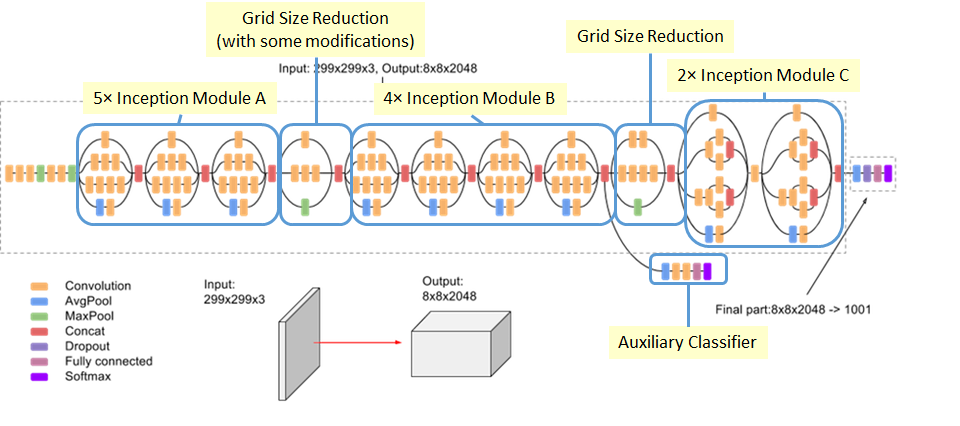
\includegraphics[width=10cm]{inception.png}
    \caption{inceptionV3}
    \label{fig:inception}
\end{figure}

\subsection{Model Comparison}
Due to its depth and the high number of fully connected layers, VGG is very slow to train and the weights are extremely large. The resulting model size may be over 500MB. However, ResNet is much deeper than VGG but the size of the model is much smaller in comparison, just a little bit over 100MB. It is becasue ResNet uses the global average pooling rather than the fully connected layers. Thus, it takes less time to train. The size of an Inception V3 model is smaller than both VGG and ResNet, no more than 100MB and trains much faster than VGG because of the use of global average pooling and Inception modules. We hope to see how our experiments in the next section will reflect the features of those models.


\section{Experiment}
\subsection{Hyperparameter Tuning}
We first tune the learning rate of three pre-trained models. Here we show the performance results of three models in terms of the training/validation loss/accuracy with learning rates of 0.00001, 0.0001, and 0.001. We use the Stochastic Gradient Descent (SGD) optimizer and Cross Entropy Loss objective function for all the models.

As we can see from Figure \ref{fig:lr_resnet} and \ref{fig:lr_vgg}, for ResNet34, the learning rate of $0.0001$ outperforms the rest of the learning rates on the validation set in terms of both accuracy and loss. The learning rate of $0.001$ is too small for the ResNet model to learn in 20 epochs. For VGG19, both learning rates of $0.00001$ and $0.0001$ have competing performance on the validation set, but the learning rate of $0.00001$ has a slightly lower validation loss and a slightly higher accuracy. Similarly, as shown in Figure \ref{fig:lr_inc}, for Inception V3, the learning rate of $0.0001$ has the best shaped curve and as well the best validation performance.
\begin{figure}[h!]
    \centering
    \begin{subfigure}{.5\textwidth}
    \centering
    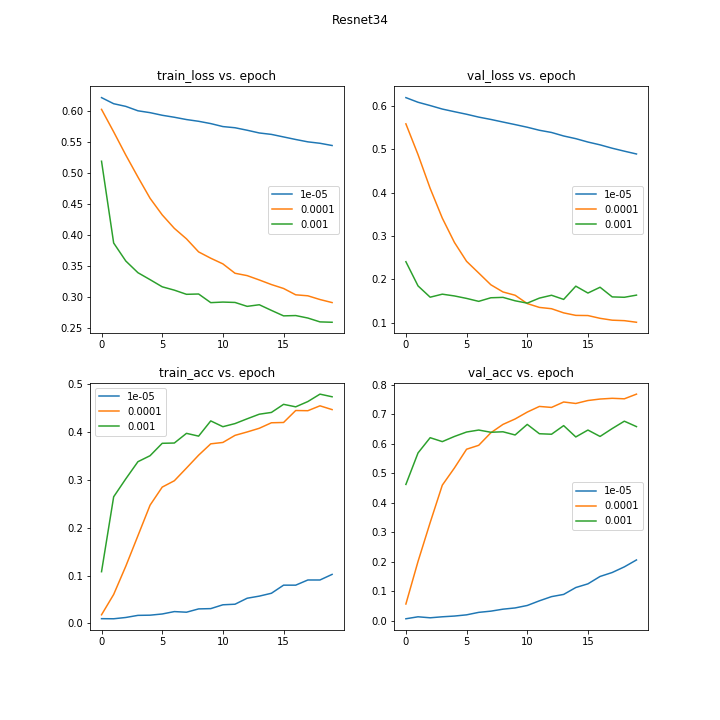
\includegraphics[height=7.5cm]{Resnet34 LR.png}
    \caption{ResNet34 Learning Rates Comparison}
    \label{fig:lr_resnet}
    \end{subfigure}%
    \begin{subfigure}{.5\textwidth}
    \centering
    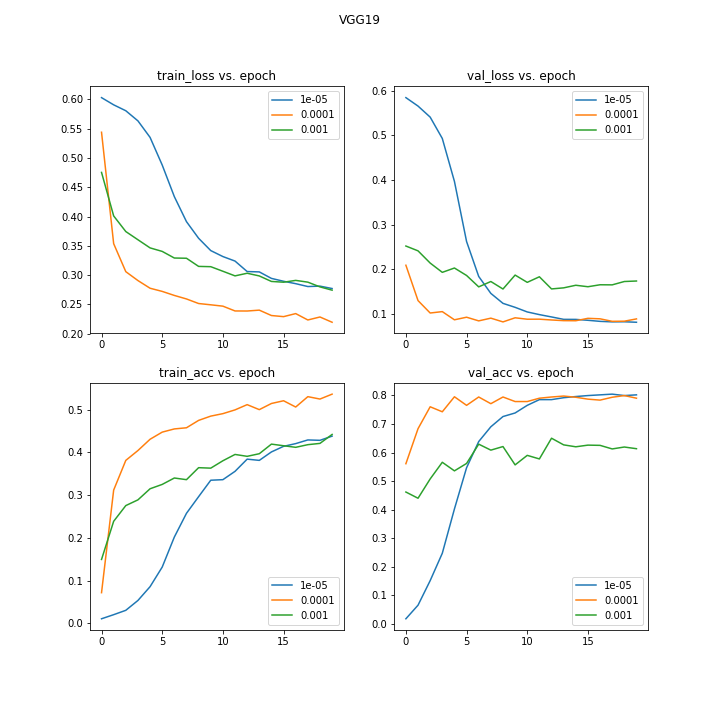
\includegraphics[height=7.5cm]{VGG19 LR.png}
    \caption{VGG19 Learning Rates Comparison}
    \label{fig:lr_vgg}
    \end{subfigure}
\end{figure}

\begin{figure}[h!]
    \centering
    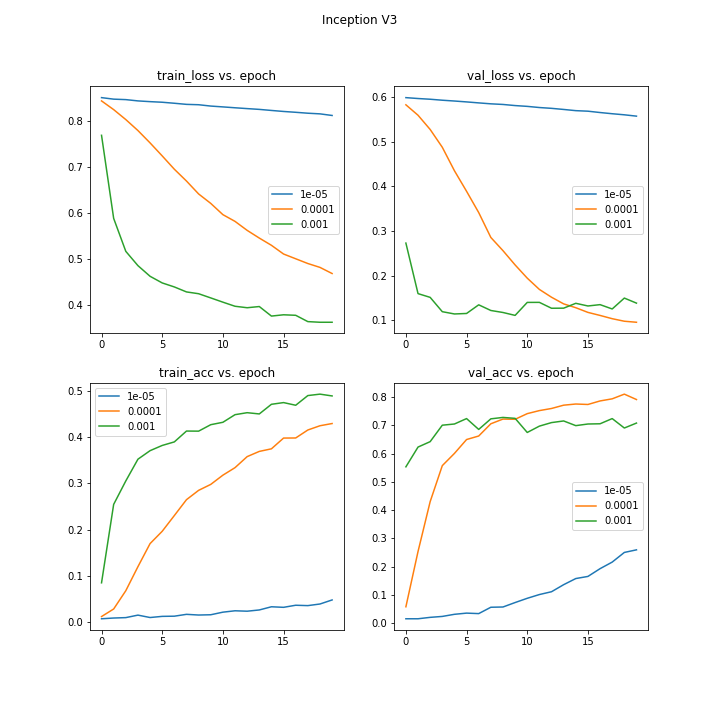
\includegraphics[height=7.5cm]{Inception V3 LR.png}
    \caption{Inception V3 Learning Rates Comparison}
    \label{fig:lr_inc}
\end{figure}

\newpage
\subsection{Partitions of the Dataset}
As mentioned earlier, we partition the original dataset into three different partitions as 60, 40, and 20 images per dog breed. For each partition of the dataset, we pick each model with best performance on the validation set and then plot the training and validation loss and accuracy curves as shown in Figure \ref{fig:60}, \ref{fig:40}, and \ref{fig:20}.

As we can see, VGG19 clearly outperforms ResNet34 and Inception V3 on both partitions of 40 and 20 images per class in terms of both validation loss and accuracy. On the partition of 60 images per class, all models have very closed performance, especially for VGG19 and Inception V3 in terms of the validation accuracy. As the general trend, more data does help the model to learn better. However, regardless of the good performance on the validation set, we still want to see the model performance on the testing test.

\begin{figure}[h!]
    \centering
    \begin{subfigure}{.5\textwidth}
    \centering
    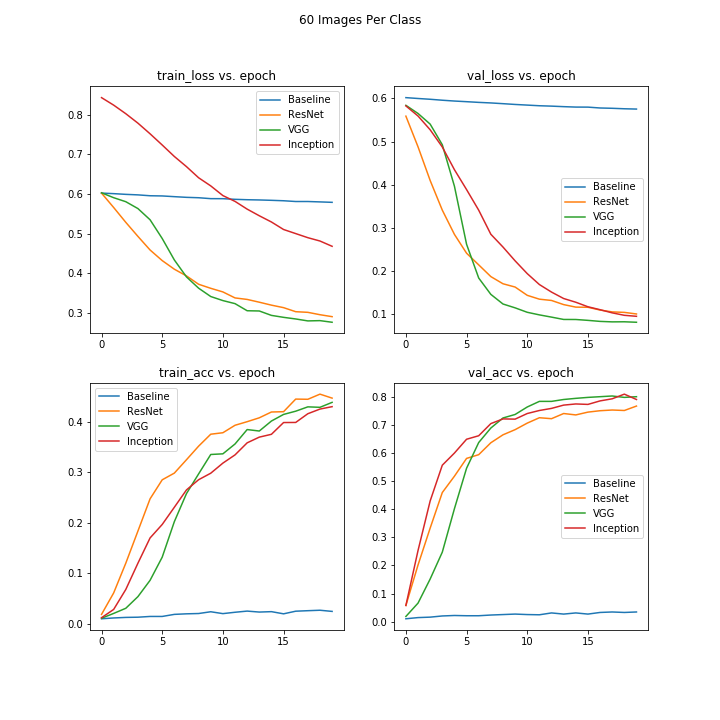
\includegraphics[height=7.5cm]{60 Images Per Class.png}
    \caption{60 Images Per Class}
    \label{fig:60}
    \end{subfigure}%
    \begin{subfigure}{.5\textwidth}
    \centering
    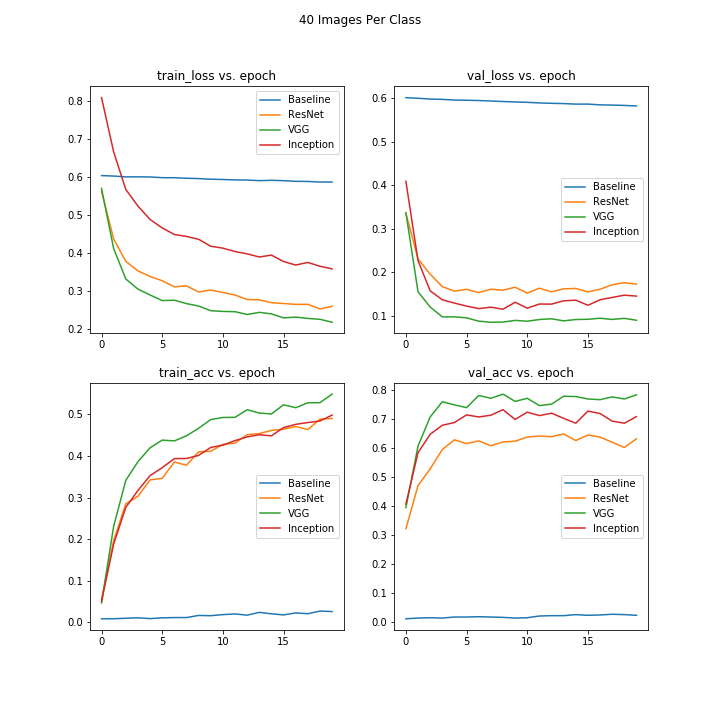
\includegraphics[height=7.5cm]{40 Images Per Class.png}
    \caption{40 Images Per Class}
    \label{fig:40}
    \end{subfigure}
\end{figure}

\begin{figure}[h!]
    \centering
    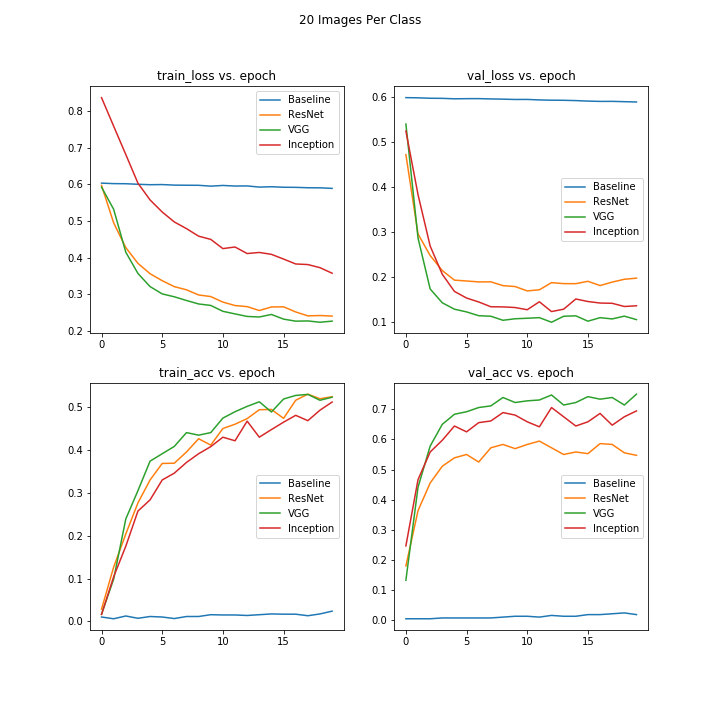
\includegraphics[height=7.5cm]{20 Images Per Class.png}
    \caption{20 Images per Class}
    \label{fig:20}
\end{figure}

\subsection{Training Time}
Table \ref{tab:spe} shows the time of each training epoch on GPU. As we can see, besides the baseline model, ResNet34 has the shortest training time per epoch and VGG19 has the longest. This matches the fact that VGG19 has a more complicated structures than the other ones and it requires more parameters to learning. By comparing the training time and test accuracy diagram, we can also verify that the longer time a model takes in training, it normally gives a more satisfying result on the testing set.

\begin{table}[h!]
    \centering
    \begin{tabular}{cccc}
         Baseline &  ResNet34 & VGG19 & Inception V3 \\
         \hline
         20.8 & 46.5 & 102.2 & 94.5 \\  
    \end{tabular}
    \caption{Second per Epoch on Partition of 60 Images Per Class}
    \label{tab:spe}
\end{table}

\subsection{Evaluation on Testing Set}
Table \ref{tab:test_acc} shows the models' accuracy on the testing set. For the baseline CNN model, it has extremely low accuracy on all three partitions, which reflects the difficulty of this classification task. VGG19 stands out on smaller dataset (20 and 40 partitions) but Inception V3 has the best accuracy on the largest partition (60). Both ResNet34 and Inception V3 performs better with more data but VGG19 has a constant performance regardless of the size of the dataset. Concluded from above, we can say that VGG19 is more robust to smaller dataset, or remains good performance regardless of the size of the data. For other two models, more data means better performance.
\begin{table}[h!]
    \centering
    \begin{tabular}{c|cccc}
        Partition & Baseline & ResNet34 & VGG19 & Inception V3 \\
        \hline 
        20 & 0.03 & 0.61 & \textbf{0.78} & 0.71 \\
        40 & 0.03 & 0.69 & \textbf{0.75} & 0.73 \\
        60 & 0.03 & 0.75 & 0.78 & \textbf{0.80}  
    \end{tabular}
    \caption{Accuracy on Testing Set}
    \label{tab:test_acc}
\end{table}

Here we show the confusion matrix of Inception V3 on the testing set in Figure \ref{fig:cm}. We can see that most of the dog breeds can be correctly predicted with a relatively high accuracy. However, there are some darker blobs of entries showing some low accuracy among certain breeds. For example, on the bottom right corner of the confusion matrix, a cluster of breeds including Toy Poodle, Miniature Poodle, and Standard Poodle raise some confusions for the model to make the predictions. Another example is that Lhasa is more likely to be predicted as Shih-Tzu. This is because they both originate from Tibet of China and have very much alike appearance shown in Figure \ref{fig:lhasa_vs_shig}. 
\begin{figure}[h!]
    \centering
    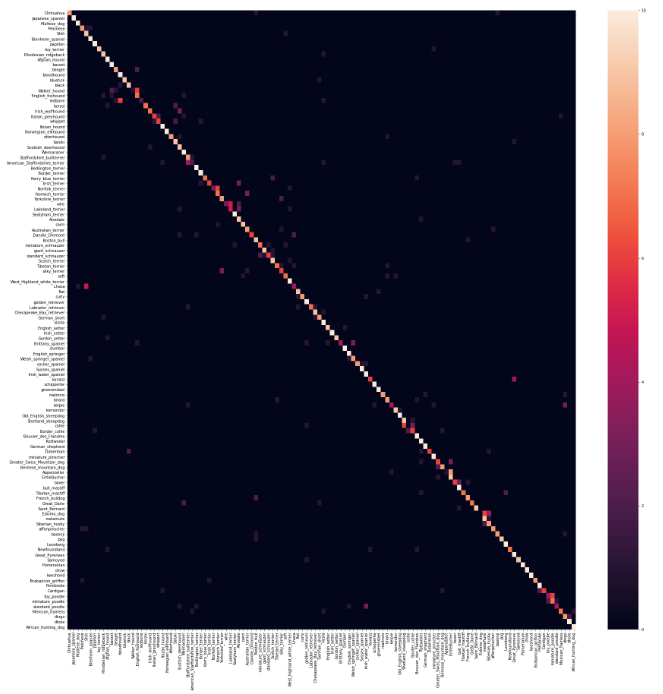
\includegraphics[width=13cm,height=11cm]{confusion_matrix_inception.png}
    \caption{Confusion Matrix on Testing Set of Inception V3}
    \label{fig:cm}
\end{figure}

\begin{figure}[h!]
    \centering
    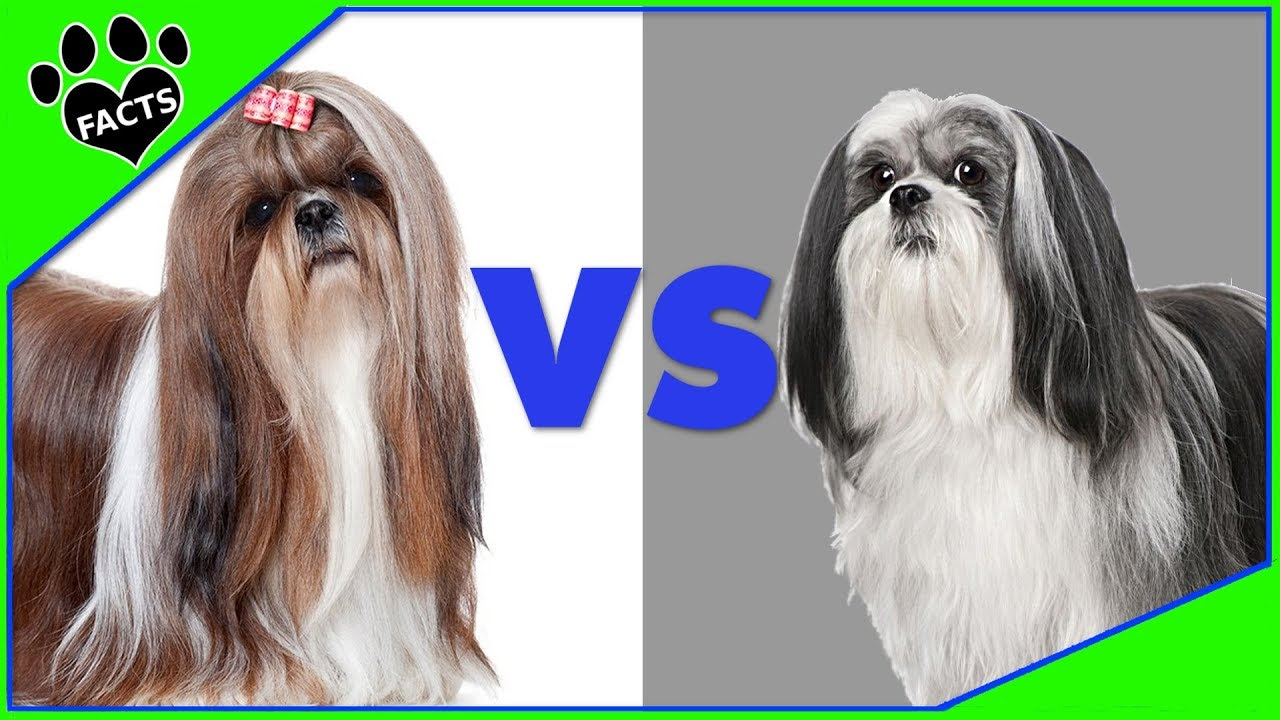
\includegraphics[width=8cm]{lhasa_vs_shih.jpg}
    \caption{Lhasa vs. Shih-Tzu}
    \label{fig:lhasa_vs_shig}
\end{figure}

\subsection{Evaluation on Unseen Dog Images}
To further test model's performance on dog images outside the original dataset, we feed some dog images collected from the internet and here are some examples. As shown in Figure \ref{fig:correct_pred}, both dog breeds are predicted correctly. However, as shown in Figure \ref{fig:wrong_pred}, an Appenzeller is predicted as a Greater Swiss Mountain Dog possibly due to the fact that both dog breeds are variations of one common origin.

\begin{figure}[h!]
    \centering
    \begin{subfigure}{.5\textwidth}
    \centering
    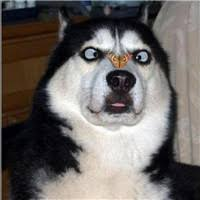
\includegraphics[width=4cm,height=4cm]{husky.jpg}
    \caption{Husky Predicted as Siberian Husky}
    \label{fig:husky}
    \end{subfigure}%
    \begin{subfigure}{.5\textwidth}
    \centering
    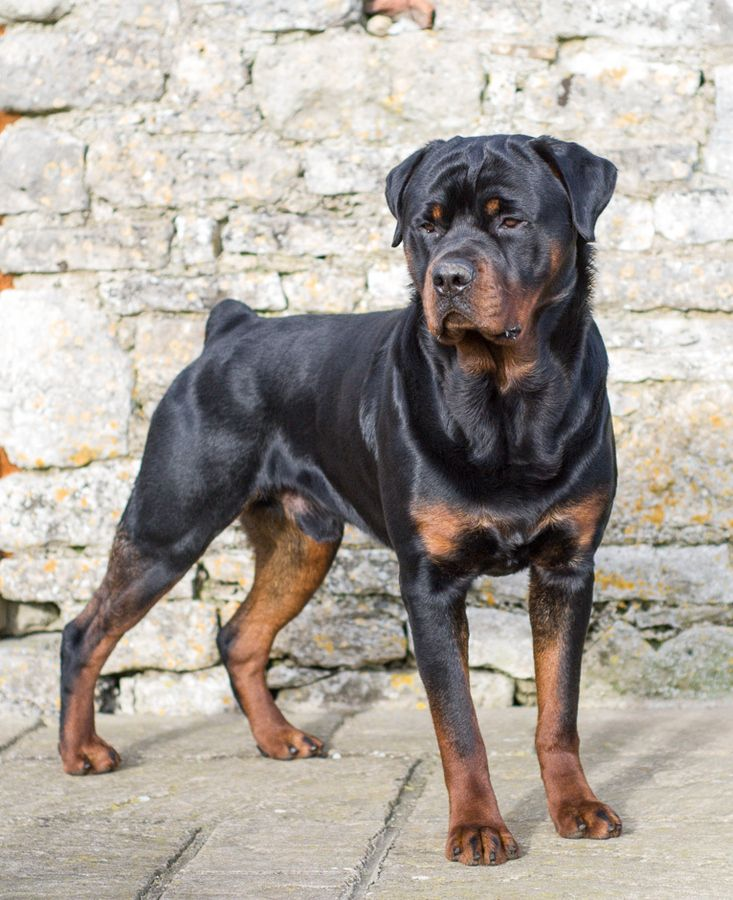
\includegraphics[width=4cm,height=4cm]{Rottweiler.jpg}
    \caption{Rottweiler predicted as Rottweiler}
    \label{fig:rott}
    \end{subfigure}
    \caption{Correct Predictions}
\label{fig:correct_pred}
\end{figure}

\begin{figure}[h!]
    \centering
    \begin{subfigure}{.5\textwidth}
    \centering
    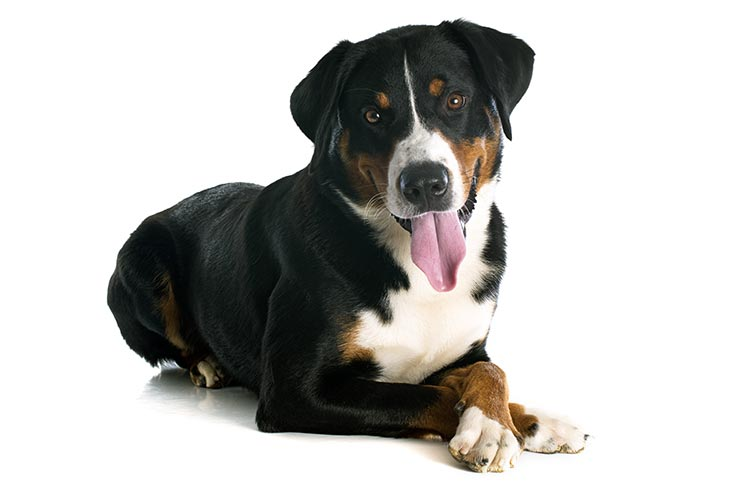
\includegraphics[width=4cm,height=4cm]{Appenzeller.jpg}
    \caption{Appenzeller Predicted as Greater Swiss Mountain Dog}
    \label{fig:husky}
    \end{subfigure}%
    \begin{subfigure}{.5\textwidth}
    \centering
    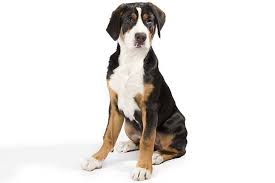
\includegraphics[width=4cm,height=4cm]{gsmd.jpg}
    \caption{A Greater Swiss Mountain Dog}
    \label{fig:rott}
    \end{subfigure}
    \caption{Wrong Prediction}
\label{fig:wrong_pred}
\end{figure}

\section{Application}
To extend our experiment to the actual world application, we can use the model to identify lost dogs on the street and help them return to their hosts. Thus, we run some images of the lost-dog to predict their breeds shown at Figure \ref{fig:lost}. In this way, we can identify the lost dogs from some CCTV feeds or pictures taken by some strangers to help narrow down the search radius. Another application is that we can use the classifier to help detect dog breed fraud, where some dog sellers try to fool the customers with one cheaper dog breed pretending to be an expensive one due to the similarity between two breeds.



\begin{figure}[h!]
    \centering
    \begin{subfigure}{.5\textwidth}
    \centering
    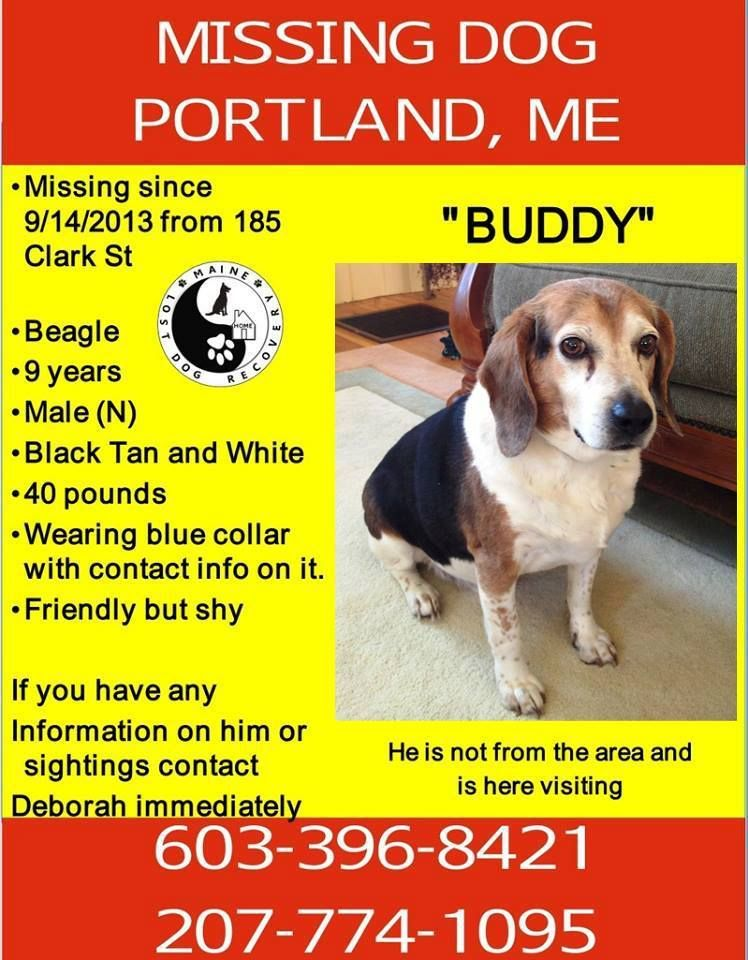
\includegraphics[width=4cm,height=5cm]{beagle.jpg}
    \caption{Predicted as Beagle}
    \label{fig:lost_beagle}
    \end{subfigure}%
    \begin{subfigure}{.5\textwidth}
    \centering
    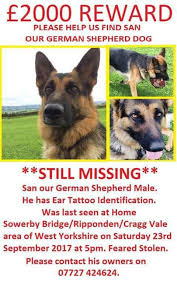
\includegraphics[width=4cm,height=5cm]{german_shepherd.jpg}
    \caption{Predicted as German Shepherd}
    \label{fig:lost_shepherd}
    \end{subfigure}
    \caption{Lost Dogs}
    \label{fig:lost}
\end{figure}

\section{Conclusion}
In our project, we apply transfer learning to identify 120 breeds of dogs and the achieve a satisfying result on the test dataset around 80 percent accuracy. 

Firstly, we apply EDA to visualize the data set distribution, then we preprocessed our data set by resizing the dataset into three dataset containing 120*20, 120*40 and 120*60 images, and we used image conversion to tensor, data augmentation,  train-val-test split before feeding into the models for training. 

In the experiment, we apply a variety of transfer learning models including CNN, VGG19, Inception V3 and ResNet34 over three datasets with different image size, we tune the parameter like the learning rate and number of epochs to find the best model with the highest validation accuracy, and we plot the loss and accuracy graph and confusion matrix to demonstrate the model performances over dataset with different image sizes.

Based on our experiments and analysis we have performed, we can majorly conclude that 
first, Inception V3 is the best model out of the four, and all transfer learning models perform significantly better than the baseline CNN model. Second, the number of image in each class does not significantly affect the model performance in transfer learning, while very limited number of images may result in a bad performance. This is because most of the low level features are already obtained in the pre-trained model. Third, most of the dog breeds can be correctly classified with Inception V3 as presenting in the confusion matrix, while only a few categories that are misclassified due to the high similarity between the two breeds. 

In the end, we decided to choose Inception V3 as our final model for dog breed prediction which runs 20 epochs with 0.0001 learning rate, Statistical Gradient Descent optimizer and Cross Entropy Loss. By applying this model on the sample test images, we can find the prediction result satisfying.

\section{Future Work}
In the future, we plan to compare the performance of some traditional machine learning methods such as Support Vector Machine and K-Nearest Neighbor. Besides, we can perform an analysis on the change of model accuracy relative to the increase of the number of Fully Connected layers added after the pre-trained model. To further improve the accuracy, we can try to add weighted Cross Entropy Loss. In addition, we can try other methods to avoid overfitting such as Learning Rate Scheduler and Early Stop; and tune other parameters such as and momentum and batch size.

\section{Contribution}
Dian Yu mainly contributes on building the VGG19, ResNet34 and Inception V3 models for transfer learning, plotting the beautiful graphs to present the learning rate tuning process, training performance of different models on three partitions of the original datasets, as well as the test result analysis and model applications. 

Zhaokai Xu mainly contributes on coming up the project idea, doing the exploratory data analysis and data preprocessing, writing the abstract, data representation and transfer learning methods description, conclusion, as well as building the baseline CNN model and preparing the project presentation.
\newpage
\bibliography{reference}
\end{document}
